%! TEX program = xelatex
% thesis_en.tex
%
% Enjoy, evolve, and share!
%
% Compile it as follows:
% xelatex demo.tex
% bibtex demo.aux
% xelatex demo.tex && xelatex demo.tex
%
% Alternatively, compile it using `make -i' (see the provided Makefile).
%
% Check file `dimscthesis.cls' for other configuration options.
%
%
% This documentclass supports the following options:
% en
% 		If present, the document adds some English pages in the front matter
% 		plus changes some headings to English. Use this option if thesis is in English.
%       Omit if written in Greek.
%
% inscr
% 		If present, then a page with the inscription provided via the command
% 		\inscription{} is printed.
%
% ack
%		If present, then a page with the acknowledgements provided via the
%		command \acksEn{} is printed.
%
% preface
%		If present, then a preface page is included just before the
%		introductory chapter. The content of this page is controled via the
%		command \preface{}.
%
% oneside
%		If present, the thesis is formatted as if it will be printed on
%		only one side of each page, the other side being left blank.
%		Default is "twoside", which is used when this option is omitted.
%
\documentclass[en,inscr,ack,preface]{dimscthesis}

% Scans for figures relative to this file
\graphicspath{ {./figures/} }

%%%%%%%%%%%%%%%%%%%%%%%%%%%%%%%%%%%%%%%%%%%%%%%%%%%%%%%%%%%%%%%%%%%%%%%%%%%%%%%
%%%%%%%%%%%%%%%%%%%% User-specific package inclusions %%%%%%%%%%%%%%%%%%%%%%%%%
%%%%%%%%%%%%%%%%%%%%%%%%%%%%%%%%%%%%%%%%%%%%%%%%%%%%%%%%%%%%%%%%%%%%%%%%%%%%%%%
\hypersetup{
    unicode=true,                     % non-Latin characters in bookmarks
    pdffitwindow=true,                % page fit to window when opened
    pdfnewwindow=true,                % links in new window
    pdfkeywords={list, of, keyword},  % list of keywords
    colorlinks=true,                  % false: boxed links; true: colored links
    linkcolor=black,                  % color of internal links
    citecolor=black,                  % color of links to bibliography
    filecolor=black,                  % color of file links
    urlcolor=black,                   % color of external links
    pdftitle={MicroRNA target prediction with novel machine learning methods beyond quadratic attention},          % title
    pdfauthor={Rafail Adam},    % author
    pdfsubject={Thesis}               % subject of the document
}
\urlstyle{same}
%%%%%%%%%%%%%%%%%%%%%%%%%%%%%%%%%%%%%%%%%%%%%%%%%%%%%%%%%%%%%%%%%%%%%%%%%%%%%%%
%%%%%%%%%%%%%%%%%%%% User-specific package inclusions %%%%%%%%%%%%%%%%%%%%%%%%%
%%%%%%%%%%%%%%%%%%%%%%%%%%%%%%%%%%%%%%%%%%%%%%%%%%%%%%%%%%%%%%%%%%%%%%%%%%%%%%%
\usepackage[shortlabels]{enumitem}
\usepackage{lscape}
\usepackage{subcaption}
\usepackage{listings}
\usepackage{csquotes}
\usepackage{float}

%%%%%%%%%%%%%%%%%%%%%%%%%%%%%%%%%%%%%%%%%%%%%%%%%%%%%%%%%%%%%%%%%%%%%%%%%%%%%%%
%%%%%%%%%%%%%%%%%%%%%% User-specific configuration %%%%%%%%%%%%%%%%%%%%%%%%%%%%
%%%%%%%%%%%%%%%%%%%%%%%%%%%%%%%%%%%%%%%%%%%%%%%%%%%%%%%%%%%%%%%%%%%%%%%%%%%%%%%
\addbibresource{references.bib}
%%%%%%%%%%%%%%%%%%%%%%%%%%%%%%%%%%%%%%%%%%%%%%%%%%%%%%%%%%%%%%%%%%%%%%%%%%%%%%%
%%%%%%%%%%%%%%%%%%%%%%%%%%% Required Metadata %%%%%%%%%%%%%%%%%%%%%%%%%%%%%%%%%
%%%%%%%%%%%%%%%%%%%%%%%%%%%%%%%%%%%%%%%%%%%%%%%%%%%%%%%%%%%%%%%%%%%%%%%%%%%%%%%
%
% First name, last name (GREEK and ENGLISH)
%
\authorFirstGr{Ραφαήλ}
\authorFirstAbrGr{Ρ.}
\authorMiddleGr{Ν.}
\authorLastGr{Αδάμ}

\authorFirstEn{Rafail}
\authorFirstAbrEn{R.}
\authorMiddleEn{N.}
\authorLastEn{Adam}
\authorSN{DSXXXXXXX}

%
% Program (greek and english)
%
\programGr{Επιστήμη Δεδομένων και Τεχνολογίες Πληροφοριών}
\programEn{Data Science and Information Technologies}

%
% The title of the thesis
%
\titleGr{Πρόβλεψη στόχων μικροRNA με νέες μεθόδους μηχανικής μάθησης πέρα από τις τετραγωνικές αρχιτεκτονικές}
\titleEn{MicroRNA target prediction with novel machine learning methods beyond quadratic attention}

%
% Month followed by Year
%
\dateGr{Οκτώβριος 2025}
\dateEn{October 2025}

%
% Advisor info
%
\advisorGr{Martin Reczko}
\advisorRankGr{Καθηγητής}
\advisorOrgGr{ΕΚΠΑ}

\advisorEn{Martin Reczko}
\advisorRankEn{Professor}
\advisorOrgEn{NKUA}

%
% Members of the advisory board
% (the first one, will be automatically taken up by the advisor)
%
\boardTwoGr{Artemis Hatzigeorgiou}
\boardTwoRankGr{Καθηγήτρια}
\boardTwoOrgGr{ΕΚΠΑ}

\boardTwoEn{Artemis Hatzigeorgiou}
\boardTwoRankEn{Professor}
\boardTwoOrgEn{NKUA}

\boardThreeGr{Panagiotis Alexiou}
\boardThreeRankGr{Καθηγητής}
\boardThreeOrgGr{ΕΚΠΑ}

\boardThreeEn{Panagiotis Alexiou}
\boardThreeRankEn{Professor}
\boardThreeOrgEn{NKUA}

%
% The examination date of the thesis
%
\examinationDateGr{Ιούνιος 2025}
\examinationDateEn{June 2025}

%
% Supervisors[heading(optional, defaluts to ΕΠΙΒΛΕΠΩΝ/SUPERVISOR)]{people} (greek and english)
%
\supervisorsGr[Επιβλέποντες]{
    {\bfseries Martin Reczko}, Καθηγητής ΕΚΠΑ {\bfseries Artemis Hatzigeorgiou}, Καθηγήτρια ΕΚΠΑ
}

\supervisorsEn[Supervisors]{
    {\bfseries Martin Reczko}, Professor NKUA {\bfseries Artemis Hatzigeorgiou}, Professor NKUA
}

%
\abstractGr{%
    Τα microRNAs είναι μικρά, μη κωδικοποιούντα μόρια RNA που συμμετέχουν σε διάφορους ρυθμιστικούς μηχανισμούς. Σε αυτή την εργασία, αναπτύσσουμε μοντέλα μηχανικής μάθησης για την πρόβλεψη αλληλεπιδράσεων μεταξύ microRNAs και στόχων mRNA. Χρησιμοποιώντας δεδομένα AGO2-eCLIP, δημιουργήσαμε ένα weighted ensemble μοντέλο που επιτυγχάνει υψηλή απόδοση σε μια ισορροπημένη κατανομή των δεδομένων κατά οικογένεια microRNA.
}

\abstractEn{%
	\par MicroRNAs are small, non-coding RNA molecules that partake in a variety of regulatory mechanisms, with the most well-studied being their role in the suppresion of translation of mRNAs via binding to sequences called MicroRNA Response Elements (MREs). They are thus implicated in a wide range of mechanisms in physiology and their disregulation can be decisive for disease states. In the current age of multi-omics analyses and personalized medicine, miRNAs are discovered via high-throughput sequencing experiments such as small RNA-seq and their regulatory roles can be studied via experiments such as AGO-eCLIP and AGO-CLASH that rely on the quantification of miRNA-mRNA hybrids. Given that a miRNA can target several different mRNA molecules, it is often complex to discern the regulatory effect of many microRNAs from a single high-throughput sequencing experiment which necessitates the use of advanced computational analyses for this purpose. To that end, several machine learning and deep learning models have emerged with the goal of miRNA target prediction. Such models aim either to predict valid miRNA-MRE pairs, or make predictions at the gene level, either finding possible MREs within the entire gene/mRNA sequence or using this information to predict changes in gene expression with the integration data from additional high-throughput sequencing experiments regarding the transriptome. The goal of this thesis is to develop a machine/deep-learning model that, given pairs of microRNAs and MREs predicts which ones would interact. For this purpose, AGO2-eCLIP data were utilized for training and evaluation of several models leading to the development of an weighted ensemble of machine learning models that is able to discern valid from invalid such pairs with an Average Precision score comparable to other state of the art models trained on the same task. The output of the model also allows for advanced interpretability via providing scores for the contribution of each feature to the final prediction.
}

%
% Subject area and keywords in Greek and English
%
\subjectAreaGr{Πρότυπο διπλωματικής εργασίας LaTeX}
\subjectAreaEn{Thesis \LaTeX{} template}

\keywordsGr{μικροRNA, πρόβλεψη στόχων, μηχανική μάθηση}
\keywordsEn{list, of, keywords}

%
% Inscription page (insc)
%
\inscription{\emph{Optional inscription section.\\
        Included when passing \emph{inscr} in the \textbackslash{}documentclass.}}

%
% Acknowledgment page (ack)
% NOTE: The dimscthesis class only supports English acknowledgements.
% To have bilingual acknowledgements, manually add Greek text to your acknowledgement content.
%
\acks{%
    Acknowledgment page. This page is optional. Included when passing the \textit{ack} option in the \textbackslash{}documentclass.
}

%
% Preface page (preface)
%
\preface{%
    This is where you provide more non-scientific details not written in the abstract or the main matter.

    This page is included by adding the \emph{preface} option in the \textbackslash{}documentclass.
}


%%%%%%%%%%%%%%%%%%%%%%%%%%%%%%%%%%%%%%%%%%%%%%%%%%%%%%%%%%%%%%%%%%%%%%%%%%%%%%%
%%%%%%%%%%%%%%%%%%%%%%%%%%%%%% Main Matter %%%%%%%%%%%%%%%%%%%%%%%%%%%%%%%%%%%%
%%%%%%%%%%%%%%%%%%%%%%%%%%%%%%%%%%%%%%%%%%%%%%%%%%%%%%%%%%%%%%%%%%%%%%%%%%%%%%%

\begin{document}

\frontmatter

\mainmatter

% add main chapters (should be given in capital letters)
\chapter{INTRODUCTION} \label{Introduction}

\section{MicroRNAs} \label{MicroRNAs}
\par MicroRNAs are the most well characterized class of non-coding RNA molecules, most commonly between 18-22 nucleotides long, that act mainly to regulate the post-transcriptional landscape of the cell, functioning as small guide RNAs for proteins of the Argonaute (AGO) family. Typically, miRNAs bind to the target mRNA sequence via their seed region which covers positions 2-8 in their sequence. Perfect complementarity leads to AGO mediated cleavage of the target with the Argonaute proteins functioning as endonucleases. Consequently, the translation of the target mRNA molecule halts and it is further targeted by other cellular RNA nucleases that lead to its complete degradation. In that manner, they are able to function in a vast variety of regulatory networks that control cellular behaviour. MicroRNAs are named based on the miRBase scheme whereby a 3-letter code denotes the species the miRNA was discovered in (e.g hsa: Homo sapiens), followed by miR in the case of mature sequences (or mir for precursor ones) and finally a number that conveys when the molecule was discovered/published with respect to the other entries \parencite{ambrosUniformSystemMicroRNA2003,kozomaraMiRBaseIntegratingMicroRNA2011}. As a rule, miRNAs from different organisms that are orthologous share the same name after the species identifier, whereas paralogous sequences have a single-letter suffix that distinguishes them and hairpin loci that give rise to the same mature miRNA are specified by a single-digit suffix. Finally, in cases where two different molecules are excised from the same precursor, a 5p or 3p suffix is used. It is also worth noting that with the advent of advanced high-throughput sequencing techniques, it has become plausible to detect isoforms of miRNAs. Such molecules differ from the canonical miRNA sequence either in terms of length of their 5' and/or 3' ends or because their sequence has been modified via processes like A-to-I or C-to-U editing. These modifications subsequently change how they are loaded to AGO and how they interact with target MREs \parencite{tomaselloMicroRNAFamilyGets2021}.

\subsection{Biogenesis} \label{Biogenesis}
\par The transcription of a miRNA gene is performed by RNA Polymerase II or RNA Polymerase III and leads to the production of a precursor called pri-miRNA which is longer in length than the mature molecule and has the structure of a stem-loop with single-stranded overhangs extending from its 3' and 5' ends. It is necessary that a stem of a pri-miRNA molecule is of specific size, its loop is at least ten base pairs long and its ends can produce single-stranded RNAs, so that it can be processed into a mature miRNA \parencite{zengSequenceRequirementsMicro2003,zhangTerminalLoopRegion2010}. The maturation process starts with a protein complex comprising of an endoribonuclease called Drosha and a protein called DGRC8. DGRC8 is a protein that binds double-stranded RNA, in this case the stem of the pri-miRNA, stabilizing its interaction with Drosha. The cleavage of the pri-miRNA by Drosha is also guided by DGRC8 which recognizes the region 11 base pairs downstream from its binding site. The product is pre-miRNA, a molecule that is 60-70 base pairs long and that is exported from the nucleus by exportin 5. An alternative origin for miRNA genes is introns of protein coding genes, such genes are also called mirtrons. Due to the fact that the pri-miRNA molecules originate from introns,they do not have the appropriate structure needed in order to be processed by Drosha and DGRC8. A protein called DRB1 solves the lariat structure of intronic RNA and pre-miRNA is the immediate product of this process. Another example of Non-canonical miRNA biogenesis includes 7-methyl Guanosine (m7G)-capped pre-miRNA, which are exported to the cytoplasm via Exportin 1 without being cleaved by Drosha first. All pre-miRNAs are recognized by a type 3 RNAse called DICER and TRBP which is a protein that binds the stem of the pre-miRNA. DICER can then cleave the pre-miRNA molecule into two leading to products of 22 base pairs long, one of which will be loaded into the RISC complex that is comprised of DICER, TRBP, AGO, PACT, and TNRC6A-C \parencite{obrienOverviewMicroRNABiogenesis2018}. 

\begin{figure}[H]
	\centering
	\begin{minipage}{0.8\linewidth}
		\centering
		% Define the figure file in the \includegraphics command
		% Must be relative to one of the paths
		% in the \graphicspath command at the top
		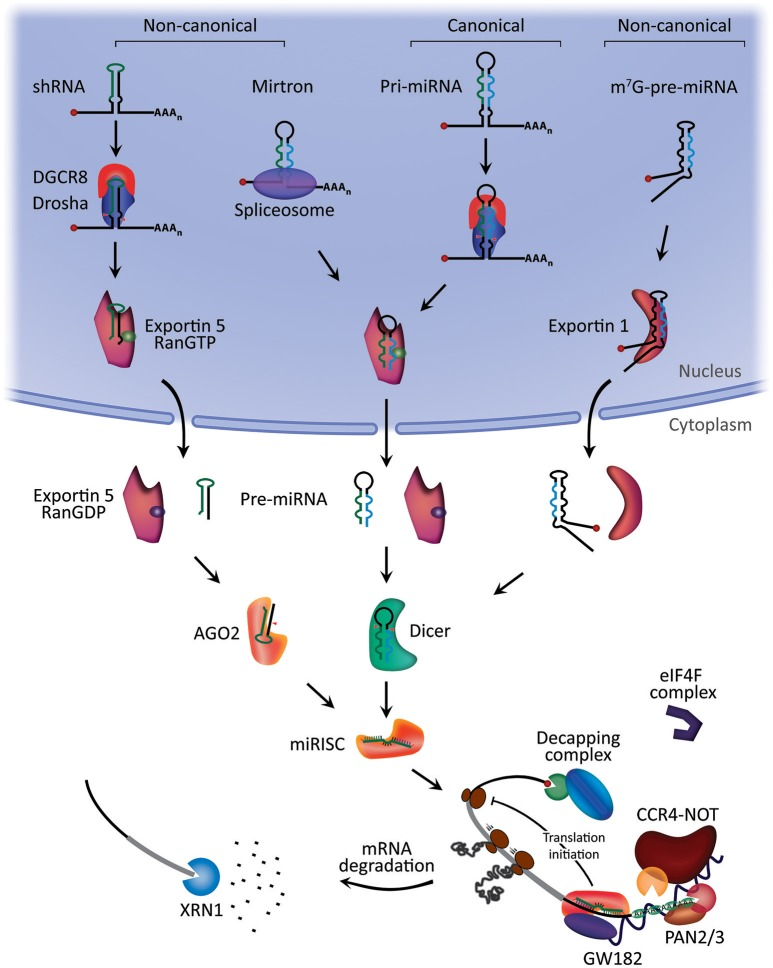
\includegraphics[width=0.9\linewidth, height=14cm]{mirbiogfunction}
		% Place caption under the figure
		\caption{The steps of miRNA biogenesis.
			\parencite{obrienOverviewMicroRNABiogenesis2018}}
		% Label the caption to include in the list of figures
		\label{fig:miRNA Biogenesis}
	\end{minipage}
\end{figure}

\subsection{Target Binding} \label{Target Binding}
\par The strand that is loaded is to be used as a guide RNA for RISC, via hybridizing with the mRNA. The dsRNA is mainly formed between the seed region of the miRNA (nucleotides 1-8) and the 3'UTR of the mRNA, with additional, downstream base pairing aiding the interaction. Given perfect complementarity, the endonuclease activity of AGO2 is induced and the mRNA is cleaved. At the same time, proteins of the GW182 complex are recruited in order to act as scaffolds for necessary effector proteins such as PAN2-PAN3 and CCR4-NOT complexes that function as Poly-A Deadenylases that remove the protective 3' polyA tail, given the interaction between tryptophan from W repeats of the GW182 complex and the PABC complex on the mRNA has been established. Finally, removal of the 5'cap of the mRNA from DCP2 takes place followed by 5'-3' degradation from the exonuclease XRN1.

Most of the miRNA:MRE complexes in the cell are not perfectly complementary and additional 3' base pairing plays an important role for their stabilization. The regulatory efficiency scales with the number of seed matches according to the following order \parencite{grimsonMicroRNATargetingSpecificity2007}:

\begin{enumerate}
	\item 8mer: 8 matches within the seed region (1-8)
	\item 7mer m8: 7 matches within the seed region (2-8)
	\item 7mer A1: 7 matches within the seed region with the first nucleotide being an Adenine (1-7)
	\item 6mer: 6 matches within the seed region (2-7)
	\item 6mer offset: 6 matches within the seed region (3-8)
	\item 5mer: 5 matches within the seed region (2-6)
\end{enumerate}

\par As mentioned above, additional base pairing can enhance the stability of the complex and is classified as supplementary binding if it does so without being necessary for the regulatory role of the miRNA, or as compensatory if it compensates for mismatches within the seed region. Finally, there is a seedless mode of pairing for miRNAs that has been described in C.elegans which likely occurs due to AU rich sequences in the seed region. Regulatory efficiency is also affected by relationships between different binding sites and binding events within the same mRNA molecule. Adjacent sites for different miRNAs and repetitive sites for the same miRNA can both function in a cooperative manner. Functional cooperativity refers to the event whereby many different binding events have a cumulative effect, whereas binding cooperativity to the physical interaction of different RISC complexes supporting each other in the binding of their target \parencite{dienerMiRNATargetInteractions2024}.

\newpage
\subsection{Additional mechanisms of action}
\par Binding of miRNAs on MREs can also increase the efficiency of translation instead of suppress it. A protein called FXR1 is necessary for this phenomenon, which in combination with RISC may bind specific sequence motifs (such as AU Rich Elements, AREs) or other sequences in the 5'UTR leading to activation of translation. MicroRNAs can also regulate gene expression via utilizing other, albeit less studied, mechanisms. For example, RISC complexes can be transported in the nucleus in order to exert regulation on transcription. In order for this to occur, they have to be imported from the cytoplasm via importin 8, importin α/β or XPO1. Within the nucleus, these complexes can bind to DNA regulatory elements affecting the binding of transcription factors and of other regulatory proteins (such as chromatin remodelling complexes) on them, thus having an impact on the transcription of related genes \parencite{kimMicroRNAdirectedTranscriptionalGene2008,chaluvally-raghavanDirectUpregulationSTAT32016,xiaoMicroRNAsActivateGene2017,guoNuclearMiR30b5pSuppresses2021}. A noteworthy example is that of miR-30b-5p which upon starvation, translocates to the nucleus in order to bind regulatory elements known as CLEAR elements that are known to bind the TFEB transcription factor. In that manner, it suppresses the transcription of these genes and inhibits lysosomal biogenesis and the autophagic flux \parencite{guoNuclearMiR30b5pSuppresses2021}. Additionally, RISC has been shown to be able to bind to mRNAs within the nucleus and induce their degradation while AGO and Drosha also participate in the splicing of premature mRNAs \parencite{obrienOverviewMicroRNABiogenesis2018}. 

\subsection{Roles in Physiology and Disease} \label{Roles in Physiology and Disease}
\par Given their diversity regarding both sequence and mechanisms of action, miRNAs partake in many physiological and pathological states. Due to their capability of regulating multiple genes in a variety of different manners, they are important components in developmental processes that require the fine-tuning of gene expression at precise time intervals, with a prominent example being that of miR-196. Anterioposterior polarity is mediated by the SHH protein in forelimb and hindlimb buds and its expression requires Retinoic Acid (RA) signalling induced Hoxb8 expression. Hoxb8 is a transcription factor protein that is upregulated as an immediate-early response to ectopic RA administration to forelimb but not to hindlimb buds due to a specific miRNA, miR-196, that inhibits the translation of Hoxb8 in a tissue specific manner \parencite{hornsteinMicroRNAMiR196Acts2005}. MicroRNAs are also able to regulate protein synthesis spatiotemporally within the cell, localizing to specific subcellular compartments before exerting their effects \parencite{corbinRoleMicroRNAsSynaptic2009}. 
\par Deregulation of miRNA expression can lead to or deteriorate a big number of disease states ranging from congenital defects to autoimmune diseases, neurological disorders and many types of cancer. For instance, \cite{adamMiR200ExpressionRegulates2009} showed that miR-200 family expression in UMUC3 cells lead to increase in E-Cadherin expression and elevated sensitivity to EGFR inhibitors. MiRNAs can also be excreted from one cell to be taken in by a target via exosomes. \cite{linBladderCancerCellsecreted2019} demonstrated that miR-21 is excreted from bladder cancer cells via exosomes that are taken in by macrophages in order to activate the PI3K/AKT pathway and promote cancer progression by polarizing them towards the M2 phenotype. In addition, miRNAs can be detected in fluid samples from patients and can thus be used as biomarkers for specific diseases. For instance, \cite{sapreUrinaryMicroRNASignature2016} showed that a combination of 6 miRNAs from urine are able to predict Urothelial Carcinoma of the Bladder (UCB) patients with a high AUC score (0.85). Finally, miRNAs can be used as targets for therapeutics that either induce or reduce their expression. An example is miR-222 which has elevated expression levels in cardiomyocytes after specific types of exercise as well as following exercise rehabilitation after heart failure. This elevated expression leads to targeting of p27, HIPK-1, HIPK-2, and HMBOX1 which promotes cardiomyocyte hypertrophy, proliferation, and survival \parencite{dingMiR222CardiovascularDiseases2017}. 

\begin{figure}[H]
	\centering
    % Define the figure file in the \includegraphics command
    % Must be relative to one of the paths
    % in the \graphicspath command at the top
    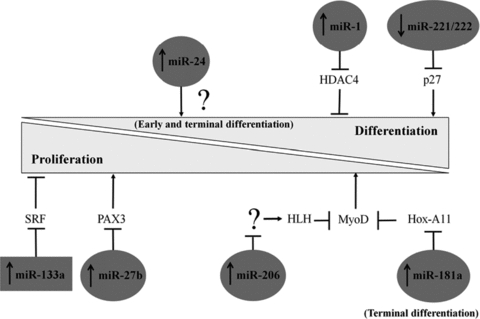
\includegraphics[width=0.7\linewidth, height=8cm]{mirmuscle}
    % Place caption under the figure
    \caption{MiRNAs regulating muscle differentiation.
        \parencite{gullerMicroRNAsSkeletalMuscle2010}}
    % Label the caption to include in the list of figures
    \label{fig: MiRNAs regulating muscle differentiation.}
\end{figure}

\subsection{High-throughput sequencing methods for miRNA research}
In the era of multiomics studies, it has become prevalent to study the totality of the miRNA part of the transcriptome as well as their targets via the use of high-throughput sequencing techniques. Such techniques allow for the detection and quantification of all the miRNA molecules in a tissue as well as of the complexes that these form with MREs. The most widely used one is small RNA-seq which includes isolation of RNA, cDNA library construction and sequencing. During RNA isolation, the total RNA might be extracted from a tissue, optionally followed by enrichment methods such as length separation or binding of small RNAs to to specific proteins. Library construction involves a reverse transcription step followed by ligation of adapters and/or polyadenylation \parencite{benesovaSmallRNASequencingApproaches2021}. The following image depicts the double ligation small RNA-seq protocol:

\begin{figure}[H]
    % Define the figure file in the \includegraphics command
    % Must be relative to one of the paths
    % in the \graphicspath command at the top
    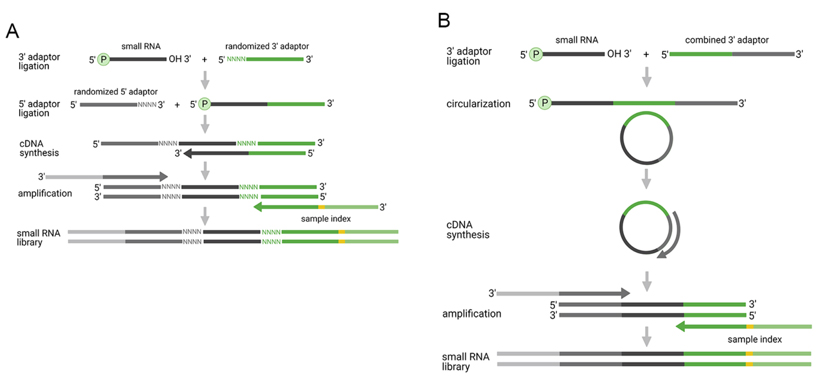
\includegraphics[width=\linewidth]{smallrnaseq}
    % Place caption under the figure
    \caption{Double ligation small RNA-seq.
        \parencite{benesovaSmallRNASequencingApproaches2021}}
    % Label the caption to include in the list of figures
    \label{fig:Double ligation small RNA-seq.}
\end{figure}

Types of experiments that capture and quantify miRNA:MRE complexes are used to study the binding sites of miRNAs and include AGO-eCLIP and AGO-CLASH. The latter involves the following steps \parencite{aMappingHumanMiRNA2013}:

\begin{figure}[H]
	\centering
	\begin{minipage}{0.8\textwidth}
		\centering
		% Define the figure file in the \includegraphics command
		% Must be relative to one of the paths
		% in the \graphicspath command at the top
		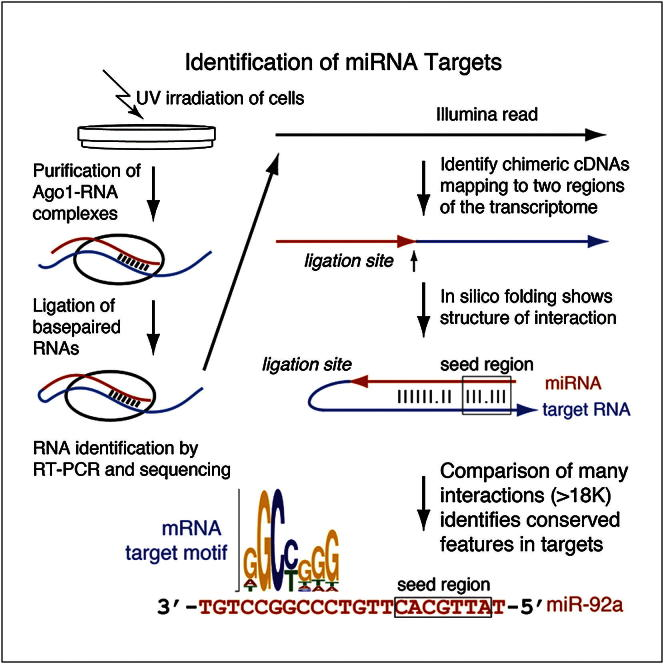
\includegraphics[width=0.8\linewidth, height=10cm]{agoclash}
		% Place caption under the figure
		\caption{AGO-CLASH.
			\parencite{aMappingHumanMiRNA2013}}
		% Label the caption to include in the list of figures
		\label{fig:AGO-CLASH}
	\end{minipage}
\end{figure}

\par Before cross-linking via UV irradiation, AGO expression is induced via the use of Doxicyclin, where the concentration is monitored in order for AGO to be close to endogenous levels. Despite that, differences between endogenous expression do occur and with them, the risk of bias regarding specific interactions. After cross-linking, hydrolysis of interacting RNA molecules takes place followed by ligation of the hybridized miRNA:MRE duplex which creates hybrid molecules to be reverse transcribed, amplified and sequenced. AGO-eCLIP follows a different procedure that does not require modifications to the endogenous expression. During AGO-eCLIP, the RISC:MRE complex is cross-linked using UV irradiation and the RNA is fragmented in the same manner as with AGO-CLASH, then immunoprecipitation, using antibodies that bind the AGO protein, follows and ultimately ligation of the miRNA 5'-P to the mRNA's 3'-OH group along with adapter ligation to the mRNA's 5' end \parencite{manakovScalableDeepProfiling2022}. Due to the immunoprecipitation step, no exogenous induction of expression is needed, eliminating the aforementioned bias and providing an image that is more physiologically relevant.

\begin{figure}[H]
	\centering
	\begin{minipage}{0.7\textwidth}
		\centering
		% Define the figure file in the \includegraphics command
		% Must be relative to one of the paths
		% in the \graphicspath command at the top
		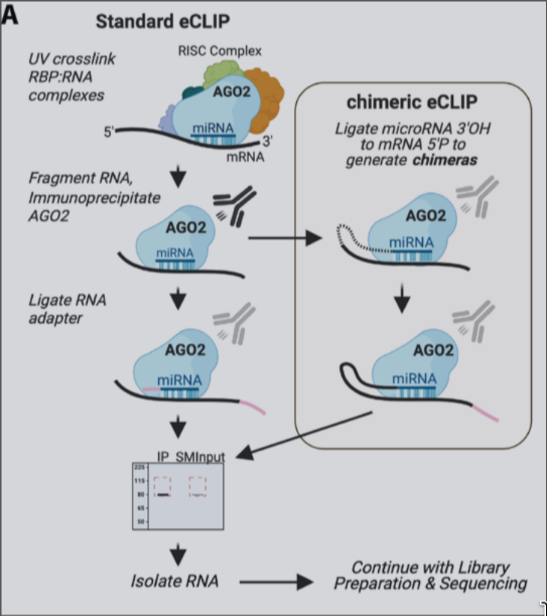
\includegraphics[width=0.8\linewidth, height=10cm]{agoeclip}
		% Place caption under the figure
		\caption{AGO-eCLIP.
			\parencite{manakovScalableDeepProfiling2022}}
		% Label the caption to include in the list of figures
		\label{fig:AGO-eCLIP}
	\end{minipage}
\end{figure}

\par There is also a family of techniques used to quantify the regulatory effect of miRNAs on their targets, which includes Degradome Sequencing, Parallel Analysis of RNA Ends and Genome-Wide Mapping of Uncapped and Cleaved Transcripts \parencite{gregoryLinkRNAMetabolism2008, addo-quayeEndogenousSiRNAMiRNA2008, germanConstructionParallelAnalysis2009}. In these experiments, the polyA transcripts are isolated from the tissue of interest, then ligation of the first adapter occurs only on transcripts with 5' monophosphate (which are the ones that have lost their 5'm7G cap due to miRNA mediated decay), followed by reverse transcription, 3' adapter ligation, PCR and sequencing. The result is depicted as a peak on an mRNA transcript where the x-axis shows the sequence the miRNA targeted and the y-axis the frequency of 5' ends found at this position.

\par High-throughput sequencing techniques produce enormous amounts of data regardless of their end goal. Commonly, the immediate result from the sequencing instrument involves files that are called FASTQ files which include entries of all the sequenced molecules along with a quality score that conveys the reliability of the base that was sequenced at a given position. Each entry of a FASTQ file follows the format below:
\begin{enumerate}
	\item 1st Line: @ character followed by an identifier for the entry
	\item 2nd Line: Raw nucleotide seq
	\item 3rd Line: + character optionally followed by the sequence identifier again
	\item 4th Line: quality values for the sequence
\end{enumerate}

\par It is worth noting that there is a number of different sequencing instruments that can be used for the same protocol but utilize different biochemistry principles in order to perform sequencing at such large scales. Due to these differences, the end result will be different even if one were to sequence the exact same samples and as such specific methods have been developed to mitigate this issue and ensure reproducibility across studies. Such methods are necessary when one wants to combine results from a number of different studies that have performed these experiments and the process called Batch Effect Correction. Finally, even within the same experiment it is heavily suggested that there are more than one replicates for the same sample in order to account for technical variation in the measurements.

\par Depending on the sequencing protocol and the end goal, these files are processed following different pipelines which include the usage of a series of computational tools. A common step regardless of the protocol is the Quality Control step (QC) in which various plots are produced in order to examine the integrity of the sequenced molecules based on the quality scores themselves as well as knowledge regarding the expected nucleotide and length distributions. Depending on the results, the next step involves filtering based on specific thresholds and optional removal of the adapter sequences followed by another QC step to ensure integrity has been maintained.

\par The next step is to map the sequences in the filtered file on the human genome/transcriptome and it is the first source of heterogeneity pertaining to such pipelines. Tools that perform this mapping are called Aligners and there is a big number of such tools each of which excels in specific circumstances. For small RNA-seq, two aligners that are commonly used are Bowtie2 and BWA-MEM \parencite{langmeadUltrafastMemoryefficientAlignment2009,liAligningSequenceReads2013}, that achieve high speed alignment of short reads on genomic sequences. The choice of the alignment tool as well as that of its alignment parameters are vital for the quality of the end result which necessitates their inclusion in the pipeline for reproducibility. A vital aspect of this step is the genome version that is used where the reads are to be aligned, as different versions lead to differences in results. Most studies use hg38 which is considered the more up to date and complete version, although with deeper and more accurate sequencing more recent versions like the Telomere to Telomere version have emerged which might come to replace hg38, especially for the analysis of repetitive regions such as centromeres, telomeres and ribosomal array sequences. For AGO-eCLIP and AGO-CLASH, a typical aligner would not suffice as the reads that are sequenced are chimeric molecules, consisting partly of miRNA and of mRNA fragments. Thus, specific tools have been developed that can appropriately align each part, with an example being Hyb \parencite{travisHybBioinformaticsPipeline2014}. Hyb begins by aligning the reads either to the genome or to a known database of molecules (ideally mature mRNAs) in order to identify reads that are non-contiguously aligned and then utilizes folding algorithms to annotate the recovered duplexes.The end result is a list of RNA:RNA hybrids.

\section{miRNA Target Prediction Algorithms} \label{miRNA Target Prediction Algorithms}
\par Several methods have been developed over the years that utilize the data produced by the aforementioned experiments in order to achieve several goals related to elucidating miRNA biology. In general, predictive algorithms are separated in terms of the type of algorithms they use in order to make the prediction as well as the prediction task itself.
\begin{itemize}
	\item Algorithms
	\begin{itemize}
		\item Heuristic 
		\item Physics Based 
		\item Machine/Deep Learning 
	\end{itemize}
	\item Task
	\begin{itemize}
		\item Site Level
		\item Gene Level
		\item Functional/Pathway Level
	\end{itemize}
\end{itemize}

\par In terms of algorithms, a tool is characterized as Heuristic if it makes predictions using preset rules that are based on already discovered interactions \parencite{lewisConservedSeedPairing2005}. Such tools are considered the simplest form of prediction tools but function as a good baseline for comparison with more complex models. Physics based tools may disregard the biology behind the task and focus on expressing the problem as an energy minimization one when it comes to MRE prediction although more recent ones aim to strike a balance between using some heuristics for narrowing down some predictions in combination with energy minimization. The advancement of machine and deep learning algorithms has paved the way for the development of models that go beyond site level prediction.
\subsection{Page numbering} \label{page_numbering}

Page numbering starts at 1 from the front cover, the English title page in this case, without printing the numbers.
When printing on both sides of the sheet (two-sided by default), any blank pages are included towards the page count, but do not include any headers or footers including page numbers.
If printing on one side of the page (done by including the \emph{oneside} option in the \verb|\documentclass|), only the pages on the right are printed and any blank pages (including those on the left side) are not included towards the page count.
Numbering always finishes on the last printed page.

On two-sided theses, numbers are printed on the center of each footer.
On one-sided theses, numbers are printed on the right side of each footer.

\subsection{Page formatting} \label{page_formatting}

Pages are formatted as in this sample:

\begin{itemize}
    \item \textbf{Margins:} 2cm on all sides, plus a 0.5cm gutter on the center of the book where the pages are bound (i.e, on the left side for printed odd pages and on the right for printed even pages).
    \item \textbf{Header:} 1.25cm from the top of the page.
    Contains the title of the thesis, on the right side for odd pages, on the left for even pages, if printed two-side.
    Appears only in the main matter, that is not in the cover pages or the front matter (abstract, inscription, table of contents, ...), and not in blank pages.
    \item \textbf{Footer:} 1.25cm from the bottom of the page.
    Contains the name(s) of the author(s)
    \begin{itemize}
        \item on the right side for odd pages, on the left for even pages, if printed two-side.
        \item on the left side of all pages if printed one-side.
    \end{itemize}
    Appears only in the main matter, that is not in the cover pages or the front matter (abstract, inscription, table of contents, ...), and not in blank pages.
    \item \textbf{Page number:} included in the footer
    \begin{itemize}
        \item at the center if printed two-side.
        \item on the right if printed one-side.
    \end{itemize}
    \item \textbf{Paragraph formatting:}
    \begin{itemize}
        \item \textbf{Justification:} Justified, each non paragraph-breaking line covers the entire line width spaced as necessary.
        \item \textbf{Paragraph spacing:} 0pt for the first, 6pt between all paragraphs.
        \item \textbf{Line spacing:} 1 line.
    \end{itemize}
    \item \textbf{Font:} Arial, 12pt, Normal or Regular style
    \item \textbf{Chapter numbering:} Arial, bold, 12pt or 14 pt
    \item \textbf{Chapter title:} Arial, bold, uppercase, 14pt., centered
    \item \textbf{Section and further division title:} Arial, bold, 12pt.
    \item \textbf{Figures:} Each figure must be uniquely numbered either by chapter or by the whole document.
    They must also include a caption below them, as in this sample.
    \item \textbf{Tables:} Each table must be uniquely numbered either by chapter or by the whole document.
    They must also include a caption above them, as in this sample.
\end{itemize}

\section{Sample section}

The section title will appear in the Table of Contents.

\subsection{Sample Subsection}

The subsection title will appear in the Table of Contents.

\subsubsection{Sample subsubsection}

The subsubsection title will appear in the Table of Contents.

\paragraph{Sample paragraph}

The paragraph title will not appear in the Table of Contents.

\subparagraph{Sample subparagraph}

The subparagraph title will not appear in the Table of Contents.

\chapter{A BRIEF INTRODUCTION TO \LaTeX} \label{introduction_to_latex}

\LaTeX{} is a typesetting system.
The authors compose a \textbf{.tex} file which is then compiled to produce a document, nowadays a PDF file.
This chapter will give a brief, non-exhaustive introduction to the system.

\section{Installing \LaTeX} \label{installing_latex}

If you use macOS or Linux as your operating system, chances are \LaTeX{} is already included.
Windows does not include \LaTeX{} out-of-the-box.
If not, just install one of the following:
\begin{itemize}
    \item TeX Live (\url{https://www.tug.org/texlive/}).
    Contains a comprehensive \LaTeX{} installation with most packages included.
    Thus, it also requires a few GB worth of space in a typical installation.
    Supports most if not all packages used in this sample.
    \item MiKTeX (\url{https://miktex.org/}) is a more minimalist installation.
    Typical installations only include the essential packages, with the option of downloading more, either from the console or automatically when compiling.
    This document uses packages that are not included in the typical MiKTeX installation, but it will offer you to install them upon first compilation.
\end{itemize}

Both of these are cross-platform, they can install under Windows, macOS, or Linux.

\section{Editing} \label{editing}

\TeX{} files can be modified by any plain text processor program, such as Notepad.
Compilation to PDF is traditionally done via the terminal.
Nonetheless, it is recommended to use a dedicated \TeX{} IDE, a program designed to edit, compile and view the resulting PDF all in one program.

Some IDEs one could use to edit and compile \TeX{} files are:
\begin{itemize}
    \item \textbf{TeXworks} (\url{https://tug.org/texworks/}).
    Very basic functionality.
    This is bundled with both TeX Live and MiKTeX, so by installing any of those you don't have to install this program as well.
    \item \textbf{Texmaker} (\url{https://www.xm1math.net/texmaker/}).
    More advanced functionality.
    Includes document structure, symbol insertion, and other \LaTeX{} commands that can be added to the document with the push of a button.
    \item \textbf{TeXstudio} (\url{https://www.texstudio.org/}).
    Forked from Texmaker.
    Functions almost the same as Texmaker.
    \item \textbf{Kile} (\url{https://kile.sourceforge.io/}).
    Built by KDE.
\end{itemize}

\section{Compiling} \label{compiling}

Before we begin with the commands, I should mention that this project---either in English or Greek---uses the XeLaTeX engine to compile.
This is because while LaTeX uses the ASCII character set to typeset, XeLaTeX uses Unicode, which includes a lot more characters than ASCII.

The compilation recipe will typically consist of:
\begin{enumerate}
    \item Running xelatex
    \item Running bibtex to compile the references
    \item Running xelatex
    \item Running xelatex
\end{enumerate}

It appears that \textit{xelatex} runs a total of 3 times, once before then twice after \textit{bibtex}.
This is to ensure all \verb|\label|s have been scanned and paired with their \verb|\ref|.

\section{Formatting} \label{formatting}

\subsection{Basics} \label{basics}

Take at look at the following excerpt:

\begin{verbatim}
This is the first paragraph.
This is the next line, but is still part of the first paragraph.

This is the second paragraph. Notice the blank line between the two.
% This is a comment. Comments are not rendered in the final file.
% Comments begin with the percent symbol(%)
% and extend to the end of the line.
\end{verbatim}

In \LaTeX{}, it's rendered like this:

This is the first paragraph.
This is the next line, but is still part of the first paragraph.

This is the second paragraph. Notice the blank line between the two.
% This is a comment. Comments are not rendered in the typeset file.
% Comments begin with the percent symbol(%) and extend to the end of the line.

As we can see, if we type something onto the next line it will remain part of that paragraph.
But if we leave one line blank between texts, the next part of the text will appear on a new paragraph.

You might have also noticed that the lines starting with '\%' did not print.
That's because the \% symbol works like the // in C-inspired languages: it begins a comment until the next line.
"But wait", you might ask, "how did you type the '\%' just now"?
Simple: if you type \verb|\%| in \LaTeX{} you'll get a \% character.
Most commands begin with the backslash (\textbackslash) character, which is also used in escaping other special characters, as we'll see in \ref{escaping}.

\subsection{Escaping} \label{escaping}
Some characters like the \% are special, and behave differently in \LaTeX{} than in text documents.
For example:
\begin{itemize}
    \item The \textbf{\%} starts comments.
    \item The \textbf{\&} is used to separate columns in a row in tables.
    \item The \textbf{\textbackslash\textbackslash} either creates a new line without breaking the paragraph or starts a new row in a table environment.
    \item \textbf{\{} and \textbf{\}} to enclose into a group.
    \item \textbf{\$} to write some math.
    \item \textbf{\# \_ \~{} \^{}} as other reserved characters.
\end{itemize}

Most of these are escaped by adding the backslash character next to them (e.g. \textbackslash\&).
But to print the backslash itself, only the \verb|\textbackslash| command will print the '\textbackslash'.

\subsection{Formatting commands} \label{formatting_commands}

Some \LaTeX{} commands act like their word processor equivalents.
For example:

\begin{center}
    \begin{tabular}{c|c}
        This... & will print this \\
        \hline
        \verb|\textbf{bold}| & \textbf{bold} \\
        \verb|\textit{italics}| & \textit{italics} \\
        \verb|\underline{underline}| & \underline{underline} \\
        \verb|\textbf{\textit{bold and italics}}| & \textbf{\textit{bold and italics}}
    \end{tabular}
\end{center}

Want to center something like the table above?
Just type something like:
\begin{verbatim}
\begin{center}
    I'm a centered section!
    I start in the .tex file with \verb|\begin{center}|
    and end with \verb|\end{center}|.
\end{center}
\end{verbatim}

and you'll get:

\begin{center}
    I'm a centered section!
    I start in the .tex file with \verb|\begin{center}|
    and end with \verb|\end{center}|.
\end{center}

Want to make a list?
For unordered (bulleted) lists:
\begin{verbatim}
\begin{itemize}
    \item This is an item in an \textit{itemize} environment.
    \item Each item starts with \verb|\item|
          and continues until the next \verb|\item|
          or \verb|\end{itemize}|.
    \item You can also nest lists.
          \begin{itemize}
              \item Just open another \textit{itemize}
                    environment inside.
          \end{itemize}
\end{itemize}
\end{verbatim}

will produce:
\begin{itemize}
    \item This is an item.
    \item Each item starts with \verb|\item|
    and continues until the next \verb|\item|
    or \verb|\end{itemize}|.
\item You can also nest lists.
    \begin{itemize}
        \item Just open another \textit{itemize} environment inside.
    \end{itemize}
\end{itemize}

\clearpage

If you want to make ordered lists, with numbers:
\begin{verbatim}
\begin{enumerate}
    \item This is an ordered item
          in an \textit{enumerate} environment.
    \item It behaves like in the \textit{itemize} environment.
          But instead of bullets that are the same for each item,
          you see sequences of numbers or letters.
    \item Once again, you may nest lists.
          \begin{enumerate}
              \item Just like that.
              \item But you can go deeper:
                    \begin{itemize}
                        \item You can even nest unordered lists.
                              \begin{enumerate}
                                  \item Just how deep can this
                                        rabbit hole go?
                              \end{enumerate}
                    \end{itemize}
          \end{enumerate}
    \item Phew, back at last!
\end{enumerate}
\end{verbatim}

this is what you get:
\begin{enumerate}
    \item This is an ordered item in an \textit{enumerate} environment.
    \item It behaves like in the \textit{itemize} environment.
    But instead of bullets that are the same for each item,
    you see sequences of numbers or letters.
    \item Once again, you may nest lists.
    \begin{enumerate}
        \item Just like that.
        \item But you can go deeper:
        \begin{itemize}
            \item You can even nest unordered lists.
            \begin{enumerate}
                \item Just how deep can this rabbit hole go?
            \end{enumerate}
        \end{itemize}
    \end{enumerate}
    \item Phew, back at last!
\end{enumerate}

To add footnotes, you can do something like this:

\begin{verbatim}
Hello there!\footnote{General Kenobi!}
\end{verbatim}

to get:

Hello there!\footnote{General Kenobi!}

Want to add URLs in your document? Simple! Just type:

\begin{verbatim}
\TeX{} Users Group homepage: \url{https://www.tug.org/}
\end{verbatim}

to get:

\TeX{} Users Group homepage: \url{https://www.tug.org/}

And speaking of links, if you wish to add a bibliographical reference as it's declared in the \textbf{references.bib} file, type:

Just pay attention to the label as it is given in the corresponding \textbf{references.bib} entry.
A sample has been given in this project.
Bibliographical entries don't have to begin with "bib:", but it helps in organizing labels.

Finally, if you want to link to another reference:
\begin{verbatim}
Go to Chapter \ref{figures_and_tables}.
\end{verbatim}

will show up as:

Go to Chapter \ref{figures_and_tables}.

As you can see, this not only displays the number of the "FIGURES AND TABLES" chapter, but clicking on it navigates to the start of that chapter.
This can be used to reference anything with the \verb|\label{label_key}| command.
Just tag something with \verb|\label{key}|, then refer (link) to it with \verb|\ref{key}|.

Tables and figures are analyzed in the next sample chapter.
If you want to know more about advanced \LaTeX{} commands, there are a few tutorials online.

\subsection{Adding math equations} \label{adding_math_equations}

\LaTeX{} also supports adding math formulae and equations.
These expressions tend to use a different notation and font than the rest of the document.

There are two ways to add a math expression: \emph{inline} and \emph{display}.

In inline mode, the math expression is written on the same paragraph as the text.
For example, typing:
\begin{verbatim}
One of Albert Einstein's famous equations is \(E = mc^2\),
where \(E\) is energy,
\(m\) is mass,
\(c\) is the speed of light (approx. 300,000,000 m/s).
\end{verbatim}

will yield:

One of Albert Einstein's famous equations is \(E = mc^2\),
where \(E\) is energy,
\(m\) is mass,
\(c\) is the speed of light (approx. 300,000,000 m/s).

In display mode, math expressions are rendered in their own blocks, usually centered.
For instance, if one types:
\begin{verbatim}
Ohm's law is expressed as:
\[V = I R \quad \textrm{or} \quad
I = \frac{V}{R} \quad \textrm{or} \quad
R = \frac{V}{I} \]
where \(V\) is voltage, \(I\) is current, \(R\) is resistance.
\end{verbatim}

this will output:

Ohm's law is expressed as:
\[V = I R \quad \textrm{or} \quad
I = \frac{V}{R} \quad \textrm{or} \quad
R = \frac{V}{I} \]
where \(V\) is voltage, \(I\) is current, \(R\) is resistance.

And if you want numbered equations:
\begin{verbatim}
The ideal gas law is defined as:
\begin{equation}
    p V = n R T
\end{equation}
where \(p\) is pressure of the gas,
\(V\) is the volume,
\(n\) the number of moles (not the animal kind),
\(R\) the gas constant,
\(T\) the temperature expressed in the Kelvin scale.
\end{verbatim}

to display:

The ideal gas law is defined as:
\begin{equation}
    p V = n R T
\end{equation}
where \(p\) is pressure of the gas,
\(V\) is the volume,
\(n\) the number of moles (not the animal kind),
\(R\) the gas constant,
\(T\) the temperature expressed in the Kelvin scale.

\chapter{FIGURES AND TABLES} \label{figures_and_tables}

\section{Inserting tables} \label{inserting_tables}

Below is a sample table with its caption.
Make sure you put the caption \textbf{over} the table.
For instance, this code in \LaTeX{}:

\begin{verbatim}
\begin{table}
    % this is before the table
    \caption{A sample event log, sorted by timestamp}
    % this is to label and include it in our list of tables
    \label{tbl:event_log_sample}
    \begin{center} % center the table
    \begin{tabular}{c|c|c}
        \textbf{Case Id} & \textbf{Activity} & \textbf{Timestamp} \\
        \hline
        1 & Activity A & 2021-05-24T12:30:00Z \\
        1 & Activity B & 2021-05-24T12:30:26Z \\
        1 & Activity C & 2021-05-24T12:31:04Z \\
        2 & Activity A & 2021-05-24T13:19:39Z \\
        2 & Activity B & 2021-05-24T13:19:50Z \\
        3 & Activity A & 2021-05-24T13:19:59Z \\
        2 & Activity C & 2021-05-24T13:22:14Z \\
        3 & Activity B & 2021-05-24T13:24:24Z \\
        4 & Activity A & 2021-05-24T13:25:06Z \\
        3 & Activity C & 2021-05-24T13:25:27Z \\
        4 & Activity B & 2021-05-24T13:25:53Z \\
        4 & Activity C & 2021-05-24T13:27:48Z \\
        \hline
    \end{tabular}
    \end{center}
\end{table}
\end{verbatim}

renders table \ref{tbl:event_log_sample}:

\begin{table}
    % this is before the table
    \caption{A sample event log, sorted by timestamp}
    % this is to label and include it in our list of tables
    \label{tbl:event_log_sample}
    \begin{center} % center the table
        \begin{tabular}{c|c|c}
            \textbf{Case Id} & \textbf{Activity} & \textbf{Timestamp} \\
            \hline
            1 & Activity A & 2021-05-24T12:30:00Z \\
            1 & Activity B & 2021-05-24T12:30:26Z \\
            1 & Activity C & 2021-05-24T12:31:04Z \\
            2 & Activity A & 2021-05-24T13:19:39Z \\
            2 & Activity B & 2021-05-24T13:19:50Z \\
            3 & Activity A & 2021-05-24T13:19:59Z \\
            2 & Activity C & 2021-05-24T13:22:14Z \\
            3 & Activity B & 2021-05-24T13:24:24Z \\
            4 & Activity A & 2021-05-24T13:25:06Z \\
            3 & Activity C & 2021-05-24T13:25:27Z \\
            4 & Activity B & 2021-05-24T13:25:53Z \\
            4 & Activity C & 2021-05-24T13:27:48Z \\
            \hline
        \end{tabular}
    \end{center}
\end{table}

\pagebreak

\section{Inserting figures} \label{inserting_figures}

Below is an example of inserting a figure with its caption.
Make sure you put the caption \textbf{under} the figure.
For example, this \LaTeX{} code:

\backmatter

% abbreviations table
\abbreviations
\begin{center}
    \renewcommand{\arraystretch}{1.5}
    \begin{longtable}{ l @{\qquad} l }
        \toprule
        AI    & Artificial Intelligence         \\
        SPARQL & SPARQL Protocol and RDF Query Language \\
        OWL    & Web Ontology Language                  \\
        OGC    & Open Geospatial Consortium             \\
        \bottomrule
    \end{longtable}
\end{center}

% appendix
\begin{appendix}
    % mark the beginning of the appendix
    \appendixstartedtrue

    \chapter{FIRST APPENDIX}

    \chapter{SECOND APPENDIX}

    % add appendix line to ToC
    \phantomsection
    \addcontentsline{toc}{chapter}{APPENDICES}
\end{appendix}

\printbibliography[title=REFERENCES]

\end{document}
